\chapter{Implementación} \label{chapter-implementation}
\markright{Implementación}

\paragraph{} En este capítulo se presenta el sistema de software construido para evaluar el rendimiento comparativo de las redes neuronales y SVM en términos del aprendizaje del problema HCSP.
Este sistema fue implementado utilizando \textit{Python} y la biblioteca de aprendizaje automático \textit{Scikit-Learn}, entre otras.

\paragraph{} La arquitectura del sistema está conformada por tres componentes fundamentales.
El primero es el módulo encargado de generar los datos utilizados en forma de ejemplos de entrenamiento.
Este módulo se describe en la sección \ref{chapter-implementacion:data}.
También se tiene un módulo dedicado a la generación de clasificadores, tanto redes neuronales como SVM.
Este módulo se describe en la sección \ref{chapter-implementacion:clasificadores}.
Finalmente, descrito en la sección \ref{chapter-implementacion:clasificacion}, se tiene un módulo encargado de clasificar nuevas instancias del problema.

% TODO agregar diagrama arquitectónico o algo.

\section{Generación de instancias del problema e instancias de entrenamiento} \label{chapter-implementacion:data}

\paragraph{} Dado el problema HCSP, surgen dos posibles maneras de utilizar una instancia del problema (dado por una matriz ETC) y su resolución (una planificación) en el contexto de aprendizaje automático.
Una opción implica utilizar a la matriz ETC completa como entrada del clasificador de elección y, hacer que la salida esperada sea la planificación, es decir todas las asignaciones tarea-máquina esperadas.
Esto constituye un problema de clasificación multiclase, y la desventaja principal que presenta es la de no permitir escalar en términos de máquinas o tareas.
Esto implica que si un clasificador es entrenado para aprender a resolver el problema HCSP con instancias del problema de dimensión $M \times N$, no será aplicable para ninguna otra dimensión.
La otra opción que se presenta, y la que fue escogida finalmente en este trabajo tomando como referencia el trabajo de \citet{savant-original}, es la de descomponer a una matriz ETC en varios ejemplos de entrenamiento.
Por lo tanto, dado un ejemplo de entrenamiento bajo este paradigma, se tiene a la información asociada únicamente a una tarea como la entrada, y a la asignación tarea-máquina de esa tarea como la salida esperada.
Esto causa que una instancia del problema (con su planificación asociada) de dimensión $M \times N$ se convierta en $M$ potenciales ejemplos de entrenamiento, y proporciona la posibilidad de escalar en términos de la cantidad de tareas a ejecutar.
Esta oportunidad surge dado el hecho de que ahora un ejemplo de entrenamiento está limitado únicamente por la cantidad de máquinas, y se presenta con más detalle en la sección \ref{chapter-implementacion:clasificadores}.
% matriz entera
% matriz parcial


\paragraph{} Con el objetivo de generar ejemplos de entrenamiento y validación como los discutidos anteriormente para entrenar y evaluar a los clasificadores construidos, fue necesario desarrollar un componente de software que pudiera hacerlo a demanda.
Este componente está conformado fundamentalmente por scripts, y en la Figura \ref{fig:diagrama-datos} se puede ver un diagrama de secuencia donde se explicita su funcionamiento. 

\paragraph{} Inicialmente, se utiliza un script extraído de \citet{bib-doctorado-nesmachnow} para generar instancias del problema, y se genera una solución para dicha instancia utilizando una implementación de Min-Min.
% TODO tal vez agregar implementación en apéndice.
Estos elementos son persistidos directamente al sistema de archivos de manera iterativa, de acuerdo a la cantidad de ejemplos de entrenamiento que se deseen generar.
Una vez finalizada esta etapa, es necesario modificar la estructura de los datos generados, de manera de obtener aquella estructura soportada por los clasificadores de aprendizaje automático.
Por lo tanto, se procede a tomar cada par constituido por una instancia del problema y su planificación esperada, y se generan tantos ejemplos de entrenamiento como tareas existan en la instancia del problema.
Es decir que para una instancia del problema de dimensión $M \times N$ tendremos $M$ ejemplos de entrenamiento.
Finalmente, se agrupan estos ejemplos de entrenamiento y se persisten en formato CSV para su uso posterior.
Este formato es utilizado por ser el estándar soportado más comúnmente por las librerías de manejo de datos utilizadas.

\textsc{\begin{figure}[ht!]
	\centering
    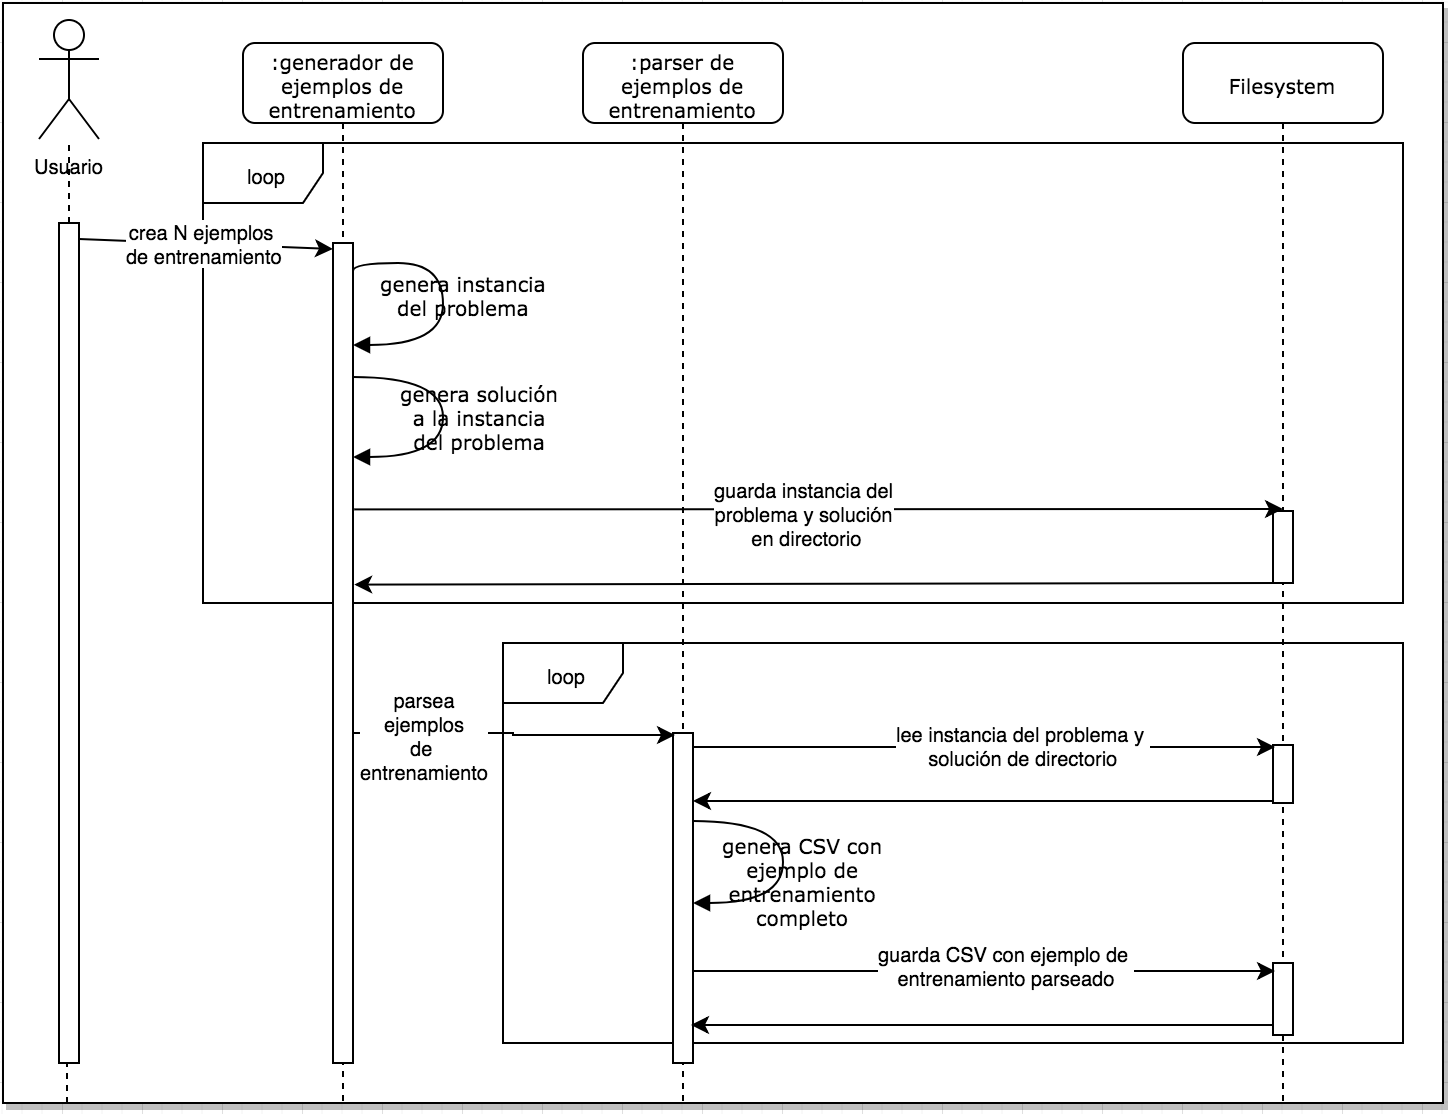
\includegraphics[width=.9\linewidth]{imagenes/implementacion/diagrama-datos.png}
	\caption{Diagrama de secuencia de generación de ejemplos de entrenamiento.}
	\label{fig:diagrama-datos}
\end{figure}}

\paragraph{} Este componente de software, como el resto de los aquí mencionados, fue desarrollado de manera de permitir su ejecución automatizada, a pesar de existir un usuario presente en el diagrama de secuencia.
Dicho usuario puede bien ser un usuario final o un script encargado de invocar a este sistema.
La posibilidad de automatización favorece la generación de ejemplos de entrenamiento a gran escala y de manera paralela mediante el uso de hilos.
Además, se ofrece al usuario la posibilidad de determinar cuántas instancias del problema (con sus correspondientes soluciones) serán generadas, dónde se persisten, y las características de los tipos de instancias del problema a generar, como por ejemplo la dimensión de las mismas.

\section{Generación de clasificadores y entrenamiento} \label{chapter-implementacion:clasificadores}

\paragraph{} Se implementó un componente de software dedicado a crear, entrenar y persistir clasificadores de aprendizaje automático. Este componente permite seleccionar como clasificador de aprendizaje automático a utilizar \textit{SVM} o redes neuronales.

\paragraph{} Se utiliza la librería \textit{Pandas}\cite{bib-pandas} de \textit{Python}. Esta librería simplifica el manejo de datos mediante estructuras de datos indizadas, proporcionando un conjunto de métodos que permiten realizar operaciones sobre éstas estructuras para facilitar el análisis de los datos, haciendo un uso eficiente de los recursos computacionales sobre los que se ejecute.

\paragraph{} Como se mencionó en la sección \ref{chapter-implementacion:data}, se utilizó cada fila de la matriz ETC del problema como los atributos para un único ejemplo de entrenamiento. Esto quiere decir que para una matriz de $512$ tareas y $16$ máquinas, se obtendrán $512$ ejemplos de entrenamiento, cada uno clasificado en una de las $16$ clases objetivo. Estas clases corresponden una a una con las máquinas asignadas por el algoritmo $Min-Min$. La figura \ref{table:datosentrenamiento} muestra un ejemplo de matriz ETC de $512$ tareas y $16$ máquinas, cada tarea con su máquina asignada siendo esta asignación la clasificación del ejemplo de entrenamiento.


\begin{figure}[ht!]
\[
\begin{bmatrix}
     & m_1 & m_2 & \dots  & m_{16} & objetivo \\
    t_1 & 35.74 & 39.62 & \dots  & 456.89 & 4 \\
    t_2 & 75.55 & 97.41a & \dots  & 579.19 & 3 \\
    \vdots & \vdots & \vdots & \vdots & \vdots & \vdots\\
    t_{512} & 130.12 & 216.59 & \dots  & 789.84 & 5\\
\end{bmatrix}
\]
\caption{Ejemplo de matriz ETC con atributo objetivo para el aprendizaje. Cada $t_i$ con $i = 1 \dots 512$ es información correspondiente a una tarea. La columna objetivo muestra la asignación de máquina para la correspondiente tarea $i$ y éste es el atributo objetivo para los clasificadores. La información asociada a la tarea, que incluye los tiempos de ejecución estimados de la tarea $t_i$ para cada una de las máquinas disponibles, junto con su clasificación, equivale a un ejemplo de entrenamiento para el clasificador.}
\label{table:datosentrenamiento}
\end{figure}

\paragraph{}A diferencia de utilizar la matriz ETC completa como ejemplo de entrenamiento, utilizar cada fila de la matriz se traduce en menores tiempos de entrenamiento y además da flexibilidad a la hora de clasificar problemas con otro número de tareas e igual número de máquinas. Esto es, como los clasificadores se entrenan con información referente a cada tarea, se pueden clasificar problemas que tengan número menor o mayor de tareas. Este tipo de escalado en función de tareas es además realista, ya que en la práctica el hardware tiende a ser una restricción menos flexible que la cantidad de tareas, algo que puede fluctuar con mayor frecuencia en función del tiempo dependiendo del caso de estudio.

\paragraph{} Para el entrenamiento se utilizaron $100$ instancias del problema de dimensión $512 \times 16$, lo que se traduce en $51200$ instancias de entrenamiento, cada una con un atributo objetivo que varía entre $1$ a $16$, siendo este el identificador de la máquina la cual la tarea es asignada. El componente de software implementado carga en memoria 100 archivos $csv$ que se encuentran en un directorio definido. Cada uno de estos archivos es una matriz ETC con el atributo objetivo correspondiente asignado para cada tarea, como se muestra en la figura \ref{table:datosentrenamiento}. Estos atributos objetivo se agregan en un sólo \textit{DataFrame}\cite{DataFrame-pandas} de \textit{Pandas}. Este \textit{DataFrame} es escalado y utilizado para el entrenamiento de los clasificadores.

\paragraph{} Debido a que los datos contienen atributos cuyas magnitudes tienen una gran varianza y los algoritmos utilizados manejan distancias euclideanas para el aprendizaje, los datos fueron escalados antes de realizarse el entrenamiento de los clasificadores. Otra razón para esclar los datos antes del entrenamiento es que \textit{Gradiente Descendente} tiende a converger más rápido cuando los datos están escalados\cite{gradiente-descendente-escalado}.

\paragraph{} El escalado de los datos se realiza mediante la clase $preprocessing.StandardScaler()$ de la librería \textit{Scikit-Learn} para \textit{Python} \cite{scikit-learn}. Esta librería provee el soporte para los métodos de aprendizaje automático y herramientas para el preprocesamiento de los datos. En particular la clase $StandardScaler()$ analiza cada atributo de manera independiente y almacena la mediana y la desviación estándar para luego ser utilizados en datos nuevos que ingresan al modelo \cite{StandardScaler-scikit-learn}.

\paragraph{} Para la construcción de los clasificadores de aprendizaje automático se utilizaron las clases \textit{svm.SVC} para la construcción de \textit{SVM} y \textit{neural\_network.MLPClassifier} para la construcción de las redes neuronales, ambas clases pertenecientes a la librería \textit{Scikit-Learn} de \textit{Python}.

\paragraph{} Con respecto al clasificador \textit{SVM}, el mismo se utilizó siguiendo la estrategia \textit{OVR}, dado que genera menos clasificadores que mediante la estrategia \textit{OVO} de acuerdo a lo expuesto en la sección \ref{capitulo:svm}. Además, se entendió \textit{OVR} como la mejor estrategia dada la baja heterogeneidad de las instancias del problema, por lo cual se espera no tener un desbalance en la cantidad de representantes de cada clase.

\paragraph{} Con respecto a las redes neuronales, en particular sobre la arquitectura de las mismas, se siguió la heurística recomendada por \citet{bib-heuristic-hobs}, dada la falta de consenso existente en la comunidad con respecto a la manera óptima de determinar la cantidad de neuronas en las capas ocultas de una red neuronal de acuerdo a los casos de uso en los que se apliquen dichos clasificadores. Según esta heurística, la cantidad de neuronas en una capa oculta (o $N_h$) se determina con la siguiente fórmula $N_h = \frac{N_s} {(\alpha * (N_i + N_o))}$, siendo:
\\
\\
$N_i$ = cantidad de neuronas de entrada
\\
\\
$N_o$ = cantidad de neuronas de salida
\\
\\
$N_s$ = cantidad de instancias de entrenamiento
\\
\\
$\alpha$ = factor de escalamiento arbitrario, con valor igual a 2 para este estudio

\paragraph{} El resto de los parámetros iniciales de configuración de la red neuronal se definieron utilizando la clase \textit{model\_selection.GridSearchCV}, que realiza una búsqueda exhaustiva de los mejores parámetros para el modelo mediante validación cruzada. A medida que se avanzó con el trabajo, estos parámetros fueron modificados para ajustarlos a las necesidades puntuales del proyecto. El detalle de los parámetros iniciales selectos se encuentra en la sección \ref{capitulo:configuracion}.
% TODO ¿agregar info sobre el clasificador usado para redes neuronales (MLPClassifier)?

% TODO la ref Pipeline-scikit-learn no figura en bibliography.bib
\paragraph{} A un nivel de abstracción superior, tanto para SVM como para redes neuronales, se utilizó la clase \textit{pipeline.Pipeline}\cite{Pipeline-scikit-learn} de la librería \textit{Scikit-Learn}. Esta clase envuelve al clasificador escogido, y permite que los datos fluyan desde su forma original, pasando secuencialmente por cada etapa del preprocesamiento, para finalmente ingresar en el clasificador. Esto permite la evaluación del modelo con estrategias como valización cruzada, simplificando la implementación del preprocesamiento de los datos mediante una encadenación de transformaciones atómicas. En particular, se utilizó un \textit{Pipeline} con el escalado encadenado al clasificador seleccionado. 

\paragraph{} Finalmente, el componente de software desarrollado se encarga de persistir los clasificadores generados. Para esto se utiliza la clase \textit{externals.Joblib} de \textit{Scikit-Learn}. El uso de \textit{Joblib} es sugerido cuando se utilizan clasificadores de \textit{Scikit-Learn}, dado que provee una manera eficiente de almacenar objetos que contienen gran cantidad de \textit{arrays} de \textit{numpy}\cite{numpy}, que es el caso de modelos de \textit{Scikit-Learn} ya entrenados.\cite{persistence}. Esta librería no solo permite la persistencia de los modelos sino que también permite la carga de los mismos en memoria para su utilización.



\newpage % orphaned line.

\section{Clasificación} \label{chapter-implementacion:clasificacion}

\paragraph{} En lo que respecta a la clasificación, se implementó un componente encargado de clasificar un conjunto de ejemplos de validación dado uno o más clasificadores ya entrenados.
Llevar a cabo esta implementación fue necesario dado que por restricciones de los recursos disponibles, evaluar el rendimiento de los clasificadores construidos mediante validación cruzada insumía una gran cantidad tiempo, limitando la agilidad del desarrollo.
Como consecuencia, se consideró como alternativa válida separar un conjunto de datos de validación a clasificar con este módulo, con el fin de obtener métricas de rendimiento de esta manera. 

\paragraph{} El componente implementado, además de disponibilizar las funcionalidades descritas anteriormente, proporciona métricas de interés adicionales.
Dentro de las métricas calculadas se encuentran el makespan esperado y el obtenido mediante predicciones.
Estas métricas son consideradas como fundamentales para evaluar el rendimiento de los clasificadores, dado que de manera independiente a la precisión, es necesario evaluar la métrica fundamental asociada al éxito de una solución del problema HCSP, que como se explica en la Sección \ref{section:descripcion-problema,subsection:estimacion-tiempo-ejecucion}, es el tiempo insumido por la máquina que finaliza su ejecución por último.
Con estos dos valores se puede evaluar qué tan exitosa fue la planificación obtenida mediante el uso de clasificadores en comparación con la solución obtenida mediante la heurística de referencia.
Finalmente, se calcula el porcentaje de ocasiones en las que el clasificador, al predecir erróneamente, escoge una máquina más rápida (constituyendo una acción ávida).
Esta métrica se calcula con el fin de evaluar si un clasificador se alejó de lo esperado en términos de precisión y makespan por haber aprendido a comportarse de manera ávida y por lo tanto aprendiendo a maximizar el beneficio local para cada tarea.

\paragraph{} La implementación del componente de clasificación consta fundamentalmente de scripts, y la Figura \ref{fig:diagrama-clasificacion} presenta un diagrama de secuencia que explicita su funcionamiento.

\newpage % orphaned line.

\paragraph{} En la implementación, inicialmente se invoca el script encargado de realizar todo este análisis sobre un conjunto de ejemplos de validación.
Estos ejemplos de validación deben estar presentes en un directorio especificado mediante opciones al invocar el script.
Posteriormente, el script invoca al script de clasificación sobre cada uno de los ejemplos de validación encontrados.
El script de clasificación se encarga de cargar el clasificador a utilizar desde una ubicación especificada del sistema de archivos.
Una vez que todas las instancias de validación se encuentran clasificadas, se efectúa el cálculo de métricas en el script de análisis.
Finalmente, el resultado es devuelto al usuario.

\textsc{\begin{figure}[ht!]
	\centering
    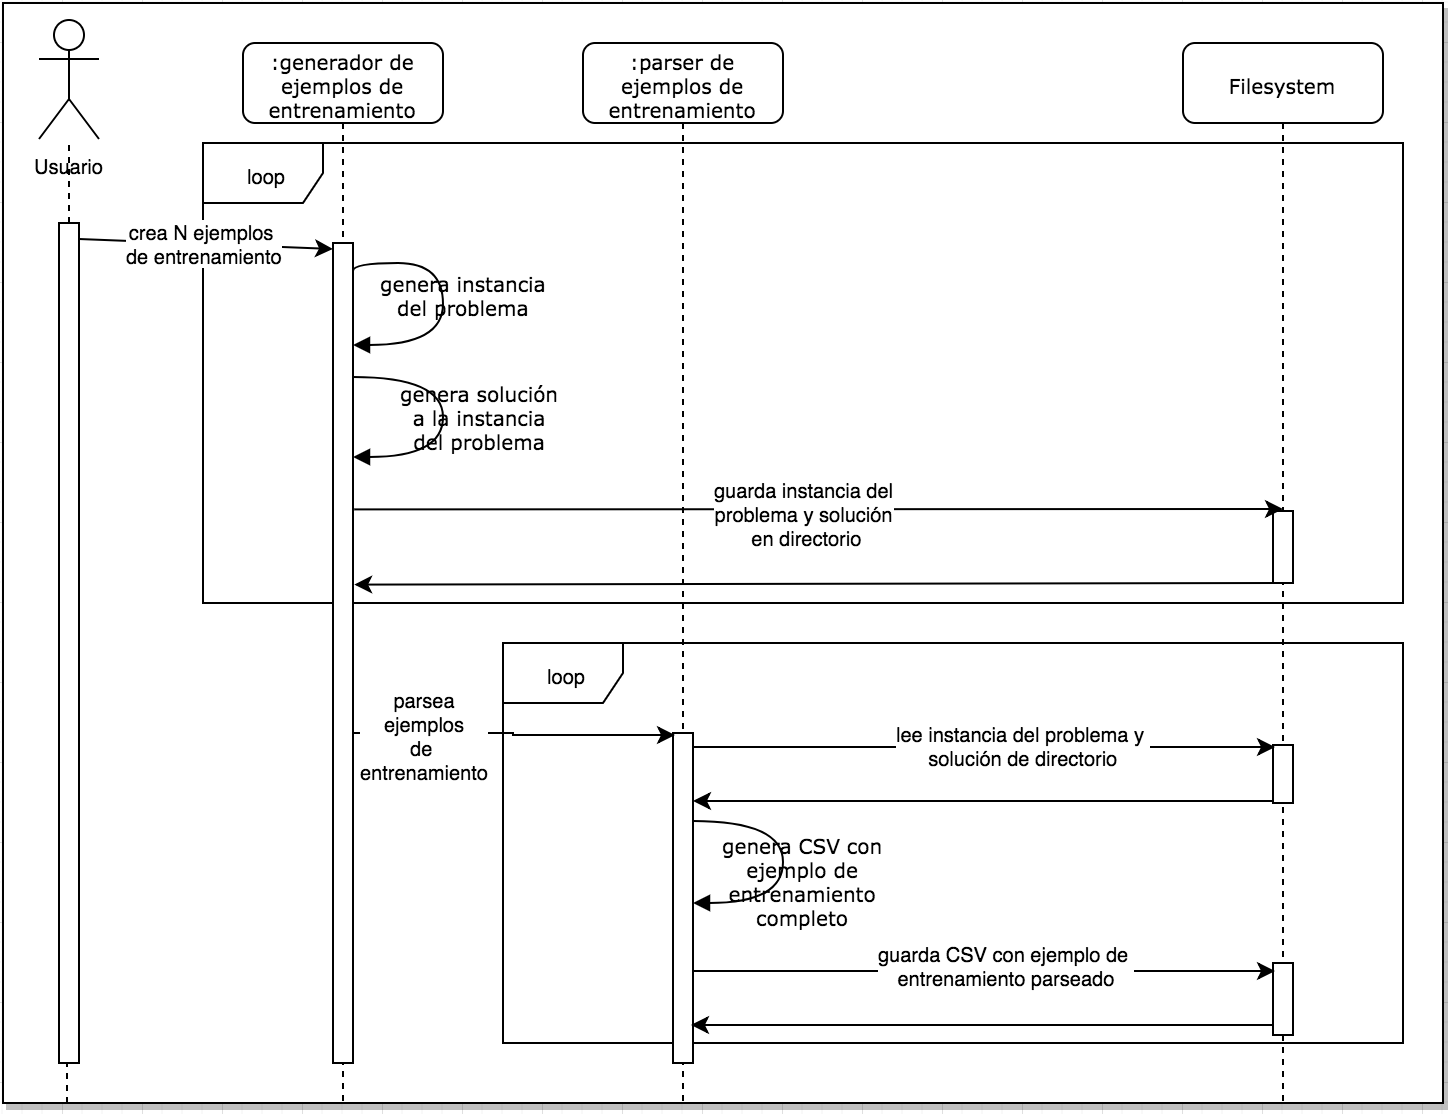
\includegraphics[width=.9\linewidth]{imagenes/implementacion/diagrama-datos.png} % TODO cambiar por validation
	\caption{Diagrama de secuencia de clasificación de ejemplos de validación.}
	\label{fig:diagrama-clasificacion}
\end{figure}}



